% -*- mode: latex; mode: visual-line; fill-column: 9999; coding: utf-8 -*-

\section{Algorithms and Software Packages}
\label{sec:packages}

For our investigation of parallel trajectory analysis we focus on using MPI as the standard approach to parallelization in HPC.
We employ the Python language, which is widely used in the scientific community because it facilitates rapid development of small scripts and code prototypes as well as development of large applications and highly portable and reusable modules and libraries.
We use the \package{MDAnalysis} library to calculate a ``RMSD time series'' (explained in section \ref{sec:mda}) as a representative use case.
Further details on the software packages are provided in sections \ref{sec:methods-mpi4py}--\ref{sec:methods-hdf5}.


\subsection{RMSD Calculation with MDAnalysis}
\label{sec:mda}

Simulation data exist in trajectories in the form of time series of atom positions and sometimes velocities.
Trajectories come in a plethora of different and idiosyncratic file formats. 
\package{MDAnalysis} \cite{Gowers:2016aa, Michaud-Agrawal:2011fu} is a widely used open source library to analyze trajectory files with an object oriented interface. 
The library is written in Python, with time critical code in C/C++/Cython. 
\package{MDAnalysis} supports most file formats of simulation packages including CHARMM \cite{Brooks:2009pt}, Gromacs \cite{Abraham:2015aa}, Amber \cite{Case:2005uq}, and NAMD \cite{Phillips:2005ek} and the Protein Data Bank \cite{Burley:2018aa} format.
At its core, it reads trajectory data in different formats and makes them available through a uniform API; specifically, coordinates are represented as standard NumPy arrays \cite{Van-Der-Walt:2011aa}.


\begin{figure}[!htb]
  \centering
  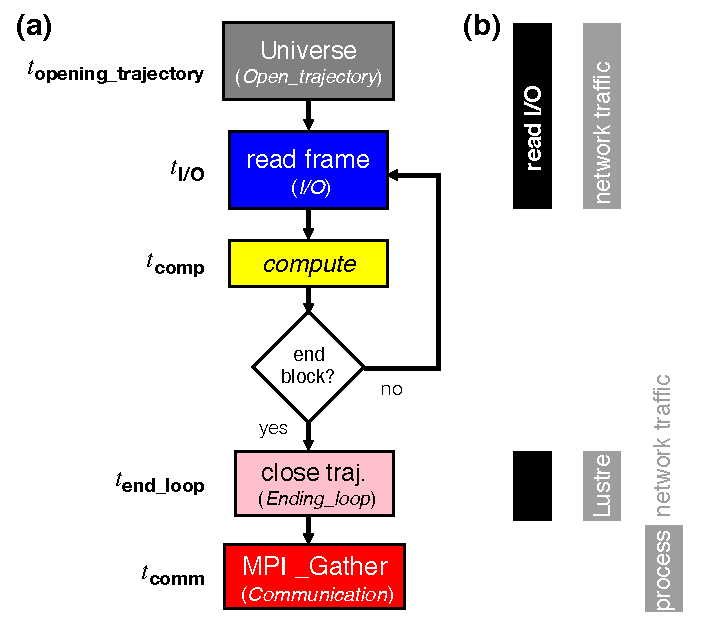
\includegraphics[width=7cm]{figures/flowchart.pdf}
  \caption{Flow chart of the MPI-parallelized RMSD algorithm, Algorithm~\ref{alg:RMSD}.
    \textbf{(a)} Each MPI process performs the same steps but reads trajectory frames from different blocks of the trajectory.
    The color scheme and labels in italics correspond to the colors and labels for measured timing quantities in the following graphs (e.g., Figs.~\protect\ref{fig:ScalingComputeIO} and \protect\ref{fig:MPIranks}).
    The names of the corresponding timing quantities from Table \protect\ref{tab:notation} are listed next to each step.
    \textbf{(b)} Steps that access the shared Lustre file system with read I/O are included in the black bars; steps that communicate via the shared InfiniBand network are included in the gray ``network traffic'' bars.
    The Lustre file system is accessed through the network and hence all I/O steps also use the network (gray ``Lustre network traffic'' bars).
    Processes only communicate over the network (gray ``process network traffic'' bar) when results are communicated back to process rank 0 in the \emph{Communication} step.
  }
  \label{fig:flowchart}
\end{figure}

As a test case that is representative of a common task in the analysis of biomolecular simulation trajectories we calculated the time series of the minimal structural root mean square distance  (\textbf{RMSD}) after rigid body superposition \cite{Lea96, Mura:2014kx}.
The RMSD is used to show the rigidity of protein domains and more generally characterizes structural changes.
It is calculated as a function of time $t$ as
\begin{equation}
  \label{eq:rmsd}
  \text{RMSD}(t) = \min_{\mathsf{R}, \mathbf{t}} %
  \sqrt{\frac{1}{N} \sum_{i=1}^{N} \left[ %
      (\mathsf{R}\cdot\mathbf{x}_{i}(t) + \mathbf{t}) - \mathbf{x}_{i}^{\text{ref}} \right]^{2}}
\end{equation}
where $\mathbf{x}_{i}(t)$ is the position of atom $i$ at time $t$, $\mathbf{x}_{i}^{\text{ref}}$ is its position in a reference structure and the distance between these two is minimized by finding the optimum $3\times3$ rotation matrix $\mathsf{R}$ and translation vector $\mathbf{t}$. 
The optimum rigid body superposition was calculated with the QCPROT algorithm~\cite{Liu:2010kx,Theobald:2005vn} (implemented in Cython and available through the \texttt{MDAnalysis.analysis.rms} module \cite{Gowers:2016aa}).

The RMSD trajectory analysis was parallelized as outlined in the flow chart in Figure~\ref{fig:flowchart}, with further details available in Algorithm~\ref{alg:RMSD}.
Each MPI process loads the core MDAnalysis data structure (called the \texttt{Universe}), which includes loading a shared ``topology'' file with the simulation system information and opening the shared trajectory file.
Each process operates on a different block of frames and iterates through them by reading the coordinates of a single frame into memory and performing the RMSD computation with them.
Once all frames in the block are processed, the trajectory file is closed and results are communicated to MPI rank 0 using \texttt{MPI\_Gather()}.

The RMSD was determined for a subset of protein atoms, the $N=146$  C$_{\alpha}$ atoms in the so-called ``core'' domain of our test system, the protein adenylate kinase \cite{Seyler:2014il} (see section \ref{sec:data} for further details).
The time complexity for the RMSD Algorithm~\ref{alg:RMSD} is $\mathcal{O}(T \times N^{2})$ where $T$ is the number of frames in the trajectory and $N$ the number of particles included in the RMSD calculation \cite{Liu:2010kx}.

\begin{algorithm}[ht]
	\scriptsize
	\caption{MPI-parallel Multi-frame RMSD Algorithm}
	\label{alg:RMSD}
	\hspace*{\algorithmicindent} \textbf{Input:} \emph{size}: total number of frames \\
	\hspace*{\algorithmicindent} \emph{ref}: mobile group in the initial frame which will be considered as reference \\
	\hspace*{\algorithmicindent} \emph{start \& stop}: starting and stopping frame index\\
	\hspace*{\algorithmicindent} \emph{topology \& trajectory}: files to read the data structure from \\
	\hspace*{\algorithmicindent} \textbf{Output:} calculated RMSD arrays
	\begin{algorithmic}[1]
		\Function{block\_rmsd}{$topology$, $trajectory$, $ref$, $index$, $start$, $stop$}                       
		\State $u \gets$ Universe$(topology$, $trajectory)$\Comment{$u$ holds all the information of the system}
		\State $g \gets$ $u.$atoms[$index$]  \Comment{select AtomGroup $g$}
		\ForAll{$iframe$ in $u.$trajectory[$start:stop$]} \Comment iterate through frames, enumerated by $iframe$
		\State $results[iframe] \gets \text{RMSD}(g, ref)$ \Comment{Eq.~\protect\ref{eq:rmsd}}
		\EndFor
		\State \Return results
		\EndFunction
		\\        
		\State MPI Init
		\State $rank \gets rank\_ID$
		\State $index \gets$ indices of the mobile AtomGroup
		\State $xref0 \gets$ reference AtomGroup position
		\State $out \gets$ \Call{block\_rmsd}{$topology, trajectory, xref0, index, start, stop$}
                \\
		\State \Call{Gather}{$out, RMSD\_data, rank\_ID=0$}
		\State MPI Finalize
	\end{algorithmic}
\end{algorithm}


\subsection{MPI for Python (\package{mpi4py})}
\label{sec:methods-mpi4py}

MPI for Python (\package{mpi4py}) is a Python wrapper for the Message Passing Interface (MPI) standard and allows any Python program to employ multiple processors \cite{Dalcin:2011aa, Dalcin:2005aa}.
Performance degradation due to using \package{mpi4py} is not prohibitive \cite{Dalcin:2011aa, Dalcin:2005aa} and the overhead is far smaller than the overhead associated with the use of interpreted versus compiled languages \cite{GAiN}.
Overheads in \package{mpi4py} are small compared to C code if efficient raw memory buffers are used for communication \cite{Dalcin:2011aa}, as used in the present study.


\subsection{MPI and Parallel HDF5}
\label{sec:methods-hdf5}

HDF5 is a structured self-describing hierarchical data format which is a common mechanism for storing large quantities of numerical data in Python (\url{http://www.hdfgroup.org/HDF5}, \cite{pythonhdf5}).
Parallel HDF5 (\package{PHDF5}) typically sits on top of a MPI-IO layer (parallel I/O with MPI) and can use MPI-IO optimizations. 
In \package{PHDF5}, all file access is coordinated by the MPI library; otherwise, multiple processes would compete over accessing the same file on disk. 
MPI-based applications launch multiple parallel instances of the Python interpreter that communicate with each other via the MPI library. 
Implementation is straightforward as long as the user supplies a MPI communicator and takes into account some constraints required for data consistency \cite{pythonhdf5}.
\package{HDF5} itself handles nearly all the details involved with coordinating file access when the shared file is opened through the \emph{mpio} driver.

MPI has two flavors of operation: collective (all processes have to participate in the same order) and independent (processes can perform the operation in any order or not at all) \cite{pythonhdf5}.
With \package{PHDF5}, modifications to file metadata must be performed collectively and although all processes perform the same task, they do not need to be synchronized \cite{pythonhdf5}. 
Other tasks and any type of data operations can be performed independently by processes.
In the present study, we use independent operations.

\begin{algorithm}[ht]
	\scriptsize
	\caption{MPI-parallel Multi-frame RMSD Algorithm with HDF5 files.}
	\label{alg:RMSDhdf5}
	\hspace*{\algorithmicindent} \textbf{Input:} \emph{size}: total number of frames \\
	\hspace*{\algorithmicindent} \emph{ref}: mobile group in the initial frame which will be considered as reference \\
	\hspace*{\algorithmicindent} \emph{start \& stop}: starting and stopping frame index\\
	\hspace*{\algorithmicindent} \emph{dataset}: HDF5 Dataset of the coordinates in the trajectory \\
	\hspace*{\algorithmicindent} \textbf{Output:} calculated RMSD arrays
	\begin{algorithmic}[1]
		\Function{$block\_rmsd$}{$dataset$, $ref$, $start$, $stop$}                       
		\For{ $start \leq iframe < stop$ }
		\State $results[iframe] \gets \Call{RMSD}{dataset[iframe], ref}$ \Comment{Eq.~\protect\ref{eq:rmsd}}
		\EndFor
		\State \Return results
		\EndFunction
		\\        
		\State MPI Init
		\State $rank \gets rank\_ID$
		\State $xref0 \gets$ reference atom group position
                \State $f \gets$ open HDF5 file for parallel MPI-IO reading \Comment{use \emph{mpio} driver}
                \State $dataset \gets$ get dataset 'pos' from $f$
		\State $out \gets \Call{block\_rmsd}{dataset, xref0, start, stop}$
                \\
		\State $\Call{Gather}{out, RMSD\_data, rank\_ID=0}$
		\State MPI Finalize
	\end{algorithmic}
\end{algorithm}

MDAnalysis does not currently have a reader for HDF5 files or HDF5-based trajectories.
In order to get a sense of the performance that is possible with a HDF5 trajectory we replaced the MDAnalysis trajectory reading in Algorithm~\ref{alg:RMSD} with directly accessing a HDF5 Dataset in a HDF5 file that was opened with the \emph{mpio} parallel driver, as shown in Algorithm~\ref{alg:RMSDhdf5}.
The HDF5 file was generated from the original XTC trajectory file as described in Section~\ref{sec:data}.